\documentclass[letterpaper]{article}
\usepackage[margin=2cm]{geometry}
\usepackage{graphicx}
\usepackage{float}
\usepackage{hyperref}

\title{Recall Manual}

\begin{document}

\maketitle
\tableofcontents

\section{Installation}

\subsection{Graphical Installation -- Simplest} \label{graphical_install}
\subsubsection{Downloading Installer}
Begin by downloading the recall\_installer.zip file. It can be found at \href{https://various-and-sundry.com/recall.html}{https://various-and-sundry.com/recall.html}.

\subsubsection{Unzipping Installer}
Navigate to the recall\_installer.zip file (example shown in figure \ref{fig:graphical_zip_file}).

\begin{figure}[H]
  \centering
  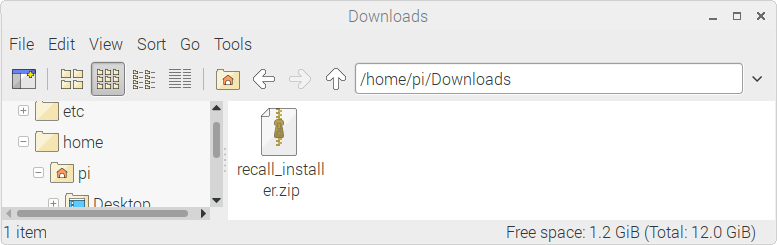
\includegraphics[width=14cm]{images/graphical_install/zip_file.png}
  \caption{\textit{recall\_installer.zip}.}
  \label{fig:graphical_zip_file}
\end{figure}

Unzip the \textit{recall\_installer.zip} file. In most desktop environments, clicking on the file with the right mouse button will display an menu containing the option 'Extract Here' (example shown in figure \ref{fig:graphical_extraction_menu}). If no 'Extract Here' option is available, the file must be extracted via another method. There may be an 'Extract To...' option, or the use of an archive program may be necessary.

\begin{figure}[H]
  \centering
  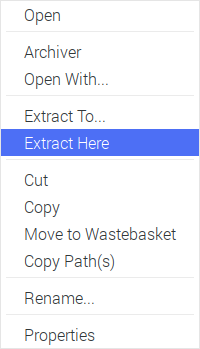
\includegraphics[width=4cm]{images/graphical_install/extraction_menu.png}
  \caption{An example menu displayed after right clicking the \textit{recall\_installer.zip}.}
  \label{fig:graphical_extraction_menu}
\end{figure}

When the contents of \textit{recall\_installer.zip} have been extracted, a directory named \textit{recall\_installer} will be created (shown in figure \ref{fig:graphical_folder_with_zip}). Click on this new directory to view its contents.

\begin{figure}[H]
  \centering
  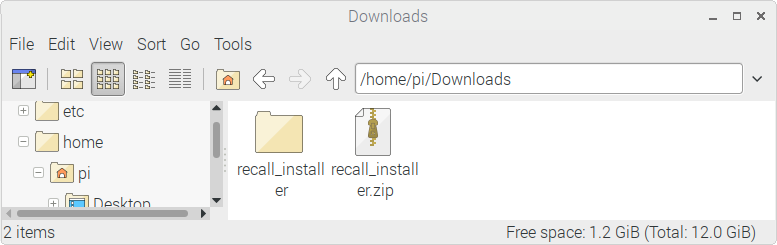
\includegraphics[width=14cm]{images/graphical_install/folder_and_zip.png}
  \caption{Extracted \textit{recall\_installer} directory alongside \textit{recall\_installer.zip}.}
  \label{fig:graphical_folder_with_zip}
\end{figure}

\subsubsection{Running Install Script}
Within the extracted \textit{recall\_installer} directory, several files will be present (as seen in figure \ref{fig:within_graphical_installer_folder}). These include the install and uninstall scripts.

\begin{figure}[H]
  \centering
  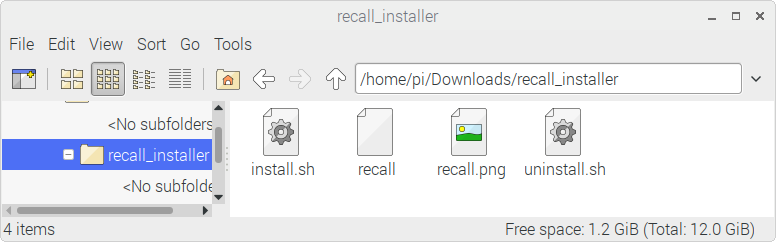
\includegraphics[width=14cm]{images/graphical_install/inside_install_folder.png}
  \caption{Contents of the \textit{recall\_installer} directory.}
  \label{fig:within_graphical_installer_folder}
\end{figure}

If the install.sh file is clicked with the right mouse button, a menu should be displayed (an example is shown in figure \ref{fig:graphical_execution_menu}. This menu should display an option to run the file (\textit{open, run, execute, etc}).

\begin{figure}[H]
  \centering
  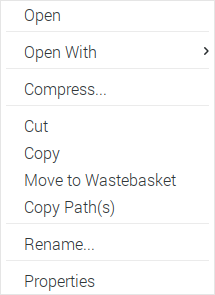
\includegraphics[width=4cm]{images/graphical_install/execution_menu.png}
  \caption{Example menu displayed after right clicking \textit{install.sh}.}
  \label{fig:graphical_execution_menu}
\end{figure}

After clicking the appropriate option, the script may execute or a prompt such as the one shown in figure \ref{fig:graphical_execution_window} may appear. Select 'Execute' or 'Execute in Terminal' to run the install script.

\begin{figure}[h]
  \centering
  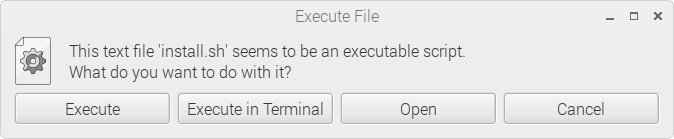
\includegraphics[width=14cm]{images/graphical_install/execution_window.png}
  \caption{Example of execution prompt.}
  \label{fig:graphical_execution_window}
\end{figure}

This script will install Recall in the \textit{\~{}/.recall} directory which will be created in the home directory. If the directory \textit{\~{}/Document} exists, the installer will create \textit{\~{}/Documents/RecallLists} to store the flashcard files. If there is no \textit{\~{}/Documents} directory, the installer will create \textit{\~{}/.recall/RecallLists} to store the flashcard files. A Recall launcher will be added to both the applications menu and the desktop. The \textit{\~{}/.recall} will also be added to the \textit{\$PATH} valuable, allowing Recall to be invoked via the command \textit{recall} (this may not work until the shell has been restarted).

\subsubsection{Potential Problems}
On some desktop environments, it may be difficult to run the install script graphically. The script may open as a plan text file instead of executing. In this case, it may be best to run the file from the command-line. Navigate into the \textit{recall\_installer} directory from the command-line and follow the instructions in section \ref{running install script in terminal}.

The install script may not work as expected on all desktop environments and/or GNU/Linux distributions. Known issues are explained in section \ref{why the install script might not work}.

\subsection{Command-Line Installation -- Most Reliable} \label{command_line_install}
\subsubsection{Downloading Installer} \label{running the install script in a terminal}
Begin by downloading the \textit{recall\_installer.zip} from \href{https://various-and-sundry.com/downloads/recall/recall_installer.zip}{https://various-and-sundry.com/downloads/recall/recall\_installer.zip}. This can be accomplished via the command \textit{wget https://various-and-sundry.com/downloads/recall/recall\_installer.zip}. This command will download the \textit{recall\_installer.zip} into the current working directory (as shown in figure \ref{fig:wget_recall_installer.zip}).

\begin{figure}[H]
  \centering
  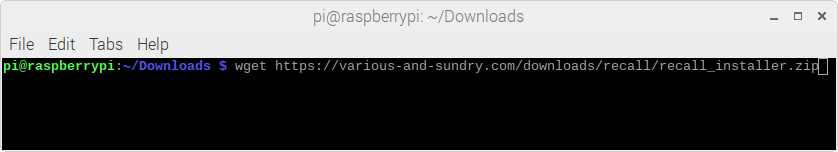
\includegraphics[width=14cm]{images/command_line_install/wget_recall_installer.png}
  \caption{Wget downloading \textit{recall\_installer.zip}.}
  \label{fig:wget_recall_installer.zip}
\end{figure}

Wget should produce a file named \textit{recall\_installer.zip} as shown in figure \ref{fig:recall_installer.zip}.

\begin{figure}[H]
  \centering
  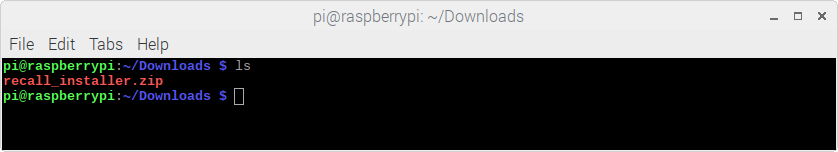
\includegraphics[width=14cm]{images/command_line_install/downloaded_zip.png}
  \caption{Downloaded installer file.}
  \label{fig:recall_installer.zip}
\end{figure}
  
\subsubsection{Unzipping Installer}

Now the installer must be unzipped. The \textit{unzip} command can be used to accomplish this. Run the command \textit{unzip recall\_installer.zip} as shown in figure \ref{fig:cammand_line_unzip}.

\begin{figure}[H]
  \centering
  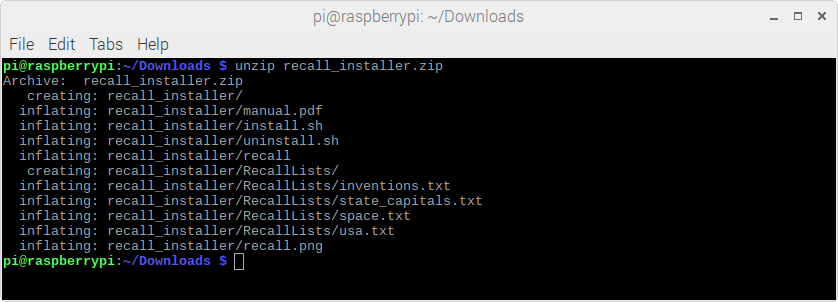
\includegraphics[width=14cm]{images/command_line_install/unzip.png}
  \caption{Unzipping \textit{recall\_installer.zip}.}
  \label{fig:cammand_line_unzip}
\end{figure}

When the extraction is finished, a directory named \textit{recall\_installer} will have been created. After running \textit{ls}, the \textit{recall\_installer} directory should be seen along with the \textit{recall\_installer.zip} (as shown in figure \ref{fig:ls_folder_and_zip}).

\begin{figure}[H]
  \centering
  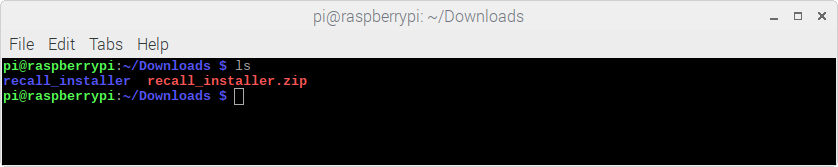
\includegraphics[width=14cm]{images/command_line_install/folder_with_zip.png}
  \caption{Extracted directory along with installer zip.}
  \label{fig:ls_folder_and_zip}
\end{figure}

Now enter the \textit{recall\_installer} directory with the command \textit{cd recall\_installer} (as shown in figure \ref{fig:cd_recall_installer}).

\begin{figure}[H]
  \centering
  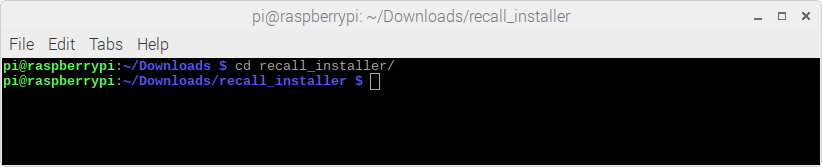
\includegraphics[width=14cm]{images/command_line_install/enter_recall_installer_folder.png}
  \caption{Entering \textit{recall\_installer} directory.}
  \label{fig:cd_recall_installer}
\end{figure}

If the command \textit{ls} is executed, the files and directories within \textit{recall\_installer} will be visible as shown in figure \ref{fig:files_in_recall_installer}. These files include the install script.

\begin{figure}[H]
  \centering
  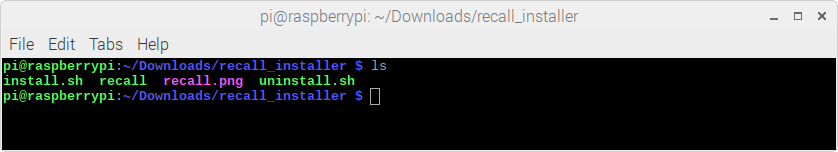
\includegraphics[width=14cm]{images/command_line_install/list_files.png}
  \caption{Files within \textit{recall\_installer} directory.}
  \label{fig:files_in_recall_installer}
\end{figure}

\subsubsection{Running Install Script} \label{running install script in terminal}
Now the install script (\textit{install.sh}) can be invoked. Bash can be directly invoke upon it by running the command \textit{bash install.sh} (as shown in figure \ref{fig:run_bash_install}). No errors were encountered if the script completes without producing any console output. The script will have installed Recall in a hidden directory in the home directory (\textit{\~{}.recall}). It will also create a directory called \textit{RecallLists} in which to store flashcard files. If the directory \textit{\~{}/Document} exists, the installer will create \textit{\~{}/Documents/RecallLists} to store the flashcard files. If there is no \textit{\~{}/Documents} directory, the installer will create \textit{\~{}/.recall/RecallLists} to store the flashcard files. A graphical launcher icon will also be added to the launch menu and the desktop. The \textit{\~{}/.recall} directory will also be added to \textit{\$PATH} variable, allowing Recall to be invoked by typing \textit{recall} into the command-line (this may not work until the shall has been restarted).

\begin{figure}[H]
  \centering
  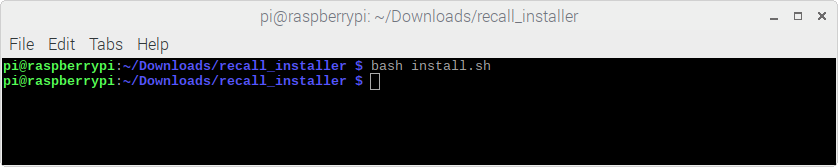
\includegraphics[width=14cm]{images/command_line_install/run_install_script.png}
  \caption{Running \textit{install.sh}.}
  \label{fig:run_bash_install}
\end{figure}

  If recall is typed into a command-line, shown in figure \ref{fig:invoke_recall_command}, Recall should start as seen in figure \ref{fig:recall_first_invoked}. This command must be invoked in a shall that was stared after the install script had finished. That is because the changes that the install script made to the \textit{\$PATH} will only be loaded in shells that were started after the install script made the changes.

  \begin{figure}[H]
    \centering
    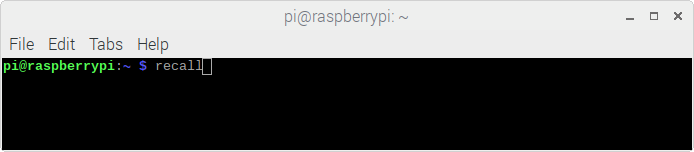
\includegraphics[width=14cm]{images/command_line_install/recall_command.png}
    \caption{Invoking Recall by typing \textit{recall}.}
    \label{fig:invoke_recall_command}
  \end{figure}

  \begin{figure}[H]
    \centering
    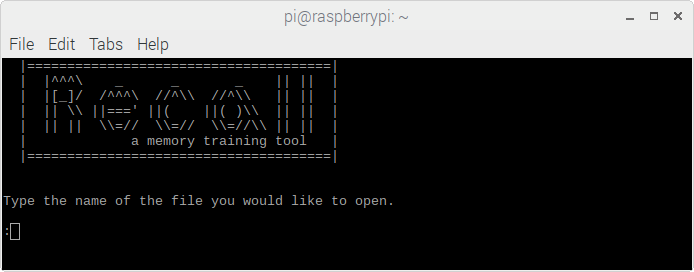
\includegraphics[width=14cm]{images/command_line_install/recall_running.png}
    \caption{Recall running.}
    \label{fig:recall_first_invoked}
  \end{figure}

\subsubsection{potential problems}
The install script may not work as expected in all desktop environments or on all GUN/Linux distributions. Potential issues are explained in section \ref{why the install script might not work}.

\subsection{Manual Install -- Not Recommended}
\subsubsection{Why Manually Install?}
Recall can be installed manually, allowing for a customized installation. This will allow the directory in which the program is stored, the launcher(s) configuration, and the \textit{\$PATH} to be manually customized. If there is no specific reason to modify these options, Recall can much more easily be installed via its install script as shown in sections \ref{graphical_install} -- Graphical Installation or section \ref{command_line_install} -- Command-Line Installation.

\subsubsection{Downloading Necessary Files}
The necessary files for installing Recall can be downloaded from \href{https://various-and-sundry.com/recall.html}{https://various-and-sundry.com/recall.html} or directly at \href{https://various-and-sundry.com/downloads/recall/recall_installer.zip}{https://various-and-sundry.com/downloads/recall/recall\_installer.zip}. Download the installer zip and extract its contents.

\subsubsection{Storing Executable}
Create a directory in which the program will be stored. By default, this would be \textit{\~{}/.recall}, but any location will work. Copy \textit{recall} and \textit{recall.png} into this directory. \textit{Recall} is the executable, and \textit{recall.png} is the icon.

The icon is not necessary for the function of Recall. It can be excluded or replaced with a different icon. If the icon is omitted, the recall logo will not appear on the program's launcher. This will not effect the program's functionality, and if you are not using a graphical environment, it will make no difference whatsoever.

\subsubsection{Adding Recall to \$PATH}
In order to run Recall from the shell, the path to the executable must be added to the \textit{\$PATH} variable. This is done by editing \textit{\~{}/.bashrc}. If recall is stored in the \textit{\~{}/.recall} directory, the following line should be added to \textit{\~{}/.bashrc}.
\begin{verbatim}
export PATH=\$PATH:~/.recall
\end{verbatim}
If the executable is stored in a different directory, this line must be changed accordingly.

\subsubsection{Creating Launchers}
This step is optional, because Recall can be launched via the command-line, but it is often useful to have a graphical launch icon.

Create a blank file with a \textit{.desktop} file extension. Under most circumstances, it makes sense to name this file \textit{Recall.desktop}, but any file name will function as long as it has a \textit{.desktop} file extension.

Within that file, add the following lines:
\begin{verbatim}
[Desktop Entry]

Type=Application
Name=Recall
Comment=A virtual flashcard tool.
Exec=bash $HOME/.recall/recall
Terminal=true
Icon=$HOME/.recall/recall.png
Categories=Education
\end{verbatim}

These options can be modified as needed. The \textit{Exec} option will need to be modified if the executable is stored in a directory other than \textit{\$HOME/.recall} or if the executable has been named something other than \textit{recall}. The \textit{Icon} option can also be changed if the location or name of the icon have been changed.

The launcher can be placed on the desktop to provide a desktop launch icon.

To add the launcher to the application launch menu, copy it into the \textit{/usr/share/applications} directory. In most desktop environments, this will add the launcher to the applications menu.

\subsection{Why the Install Script isn't Working} \label{why the install script might not work}

\subsubsection{Recall Will not Run when Invoked from the Command-Line}
If Recall's launchers work, but it will not run via a shell command (i.e. \textit{recall}), the \textit{\$PATH} variable may not include the directory in which Recall is installed (by default, \textit{\~{}/.recall}. This problem is likely caused by the install script failing to modify the \textit{\~{}/.bashrc} file correctly. Make sure that \textit{\~{}/.recall} has been added to the \textit{\$PATH} variable.

\subsubsection{Recall was not added to the Applications Menu}
This install script needs to be run by a user with sudo permission in order to add a launcher to the applications menu (i.e. \textit{/usr/share/applications}. If this permission is not provided, the install script will not be able to add a launcher to the applications menu, but it should still install recall, add it to the \textit{\$PATH}, and create a desktop launcher.

\subsubsection{No Desktop Icon}
The install script will attempt to create a desktop launcher icon by adding one to the \textit{\~{}/Desktop} directory. If this file does not exist, then this action will fail, but the rest of the installation should be successful. If the \textit{\~{}Desktop} directory exists but the desktop environment does not support desktop icons, then there will be no visible desktop icon.

\section{Using Recall}
\subsection{Basic Operation}
\subsubsection{Opening a File upon Start} \label{opening a file}
When Recall is launched, it will prompt to user to enter the name of a file (as shown in figure \ref{fig:enter_file_name}).

\begin{figure}[H]
  \centering
  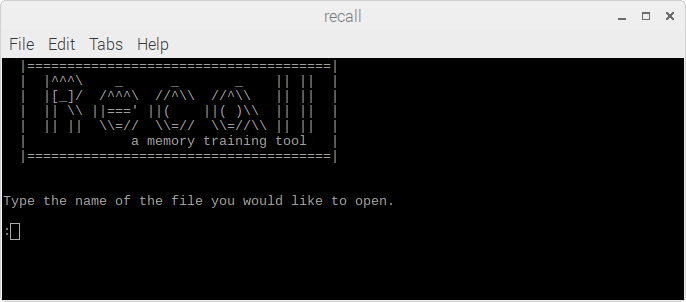
\includegraphics[width=14cm]{images/running/enter_file.png}
  \caption{Recall prompting user to enter file name.}
  \label{fig:enter_file_name}
\end{figure}

Flashcard files must be stored in a specific directory. By default, this directory will either be \textit{\~{}/Documents/RecallLists} or \textit{\~{}/.recall/RecallLists}. This directory can be changed to any other directory. Recall will access whatever directory is given in the \textit{PATH} line of the \textit{\~{}/.recall/recallrc} file. For example, if the flashcard files are stored in the \textit{\~{}/Documents/RecallLists} directory, the \textit{\~{}/.recall/recallrc} file should contain the following line.
\begin{verbatim}
PATH ~/Documents/RecallLists
\end{verbatim}

The files that contain questions and answers must have a \textit{.txt} file extension. To open one of these files, enter its name, without the \textit{.txt} extension, into Recall's file prompt. Recall will not find the file if the \textit{.txt} extension is included. Figure \ref{fig:entering_file_name} shows a file name entered into the prompt.

\begin{figure}[H]
  \centering
  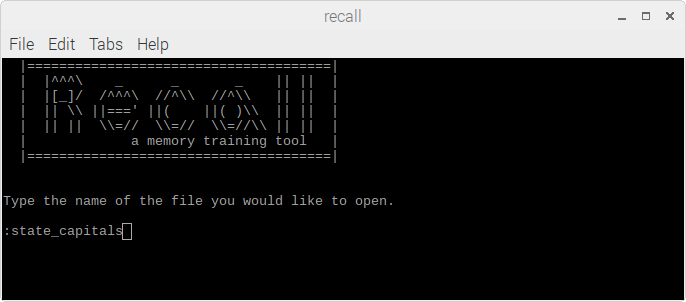
\includegraphics[width=14cm]{images/running/entered_file.png}
  \caption{Opening \textit{state\_capitals.txt}.}
  \label{fig:entering_file_name}
\end{figure}

\subsubsection{Using a Flashcard List}
Once a file has been opened in Recall, a random question from that file will be displayed (shown in figure \ref{fig:example_questian_1}). The user can then consider the question and attempt to recall the answer.

\begin{figure}[H]
  \centering
  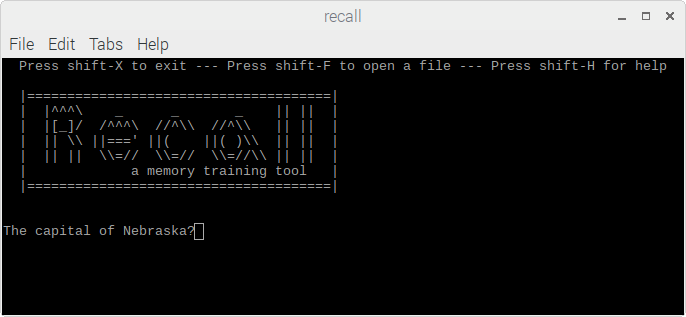
\includegraphics[width=14cm]{images/running/questian1.png}
  \caption{Example Question.}
  \label{fig:example_questian_1}
\end{figure}

Any key can be pressed to reveal the answer (as shown in figure \ref{fig:example_answer_1}). Some keys such as \textit{Home}, \textit{End}, \textit{Page Up}, \textit{Page Down}, \textit{arrows keys}, and \textit{Insert} will yield unwanted behavior, and they should be avoided.

\begin{figure}[H]
  \centering
  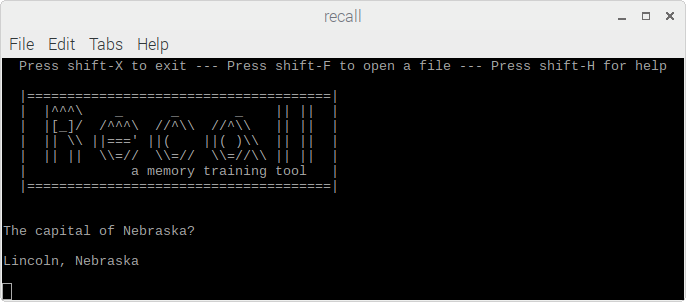
\includegraphics[width=14cm]{images/running/questian1_with_answer.png}
  \caption{Example Question with Answer}
  \label{fig:example_answer_1}
\end{figure}

Then, any key can be pressed to show another random question (shown in figure \ref{fig:example_questian_2}. Questions and answers can be cycled as quickly or slowly as the user desires.

\begin{figure}[H]
  \centering
  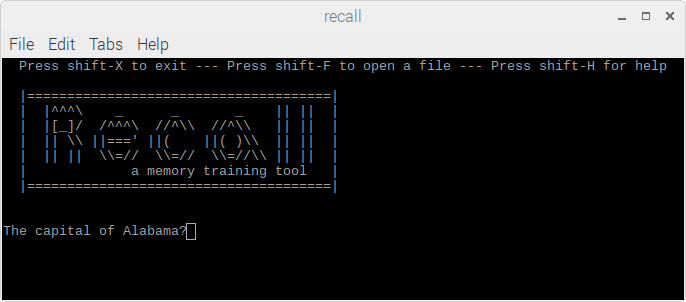
\includegraphics[width=14cm]{images/running/questian2.png}
  \caption{Another Example Question.}
  \label{fig:example_questian_2}
\end{figure}

\subsubsection{Opening a Different File}
When cycling through questions, pressing shift-\textit{f} (capital \textit{F}) will bring the user back to the file selection prompt. That allows the user to select a different flashcard file. The instructions in section \ref{opening a file} explain the process of selecting a file.

\subsubsection{Exiting}
When cycling through files, shift-\textit{x} (capital \textit{X}) will close Recall. Because Recall is a command-line application, Ctrl-\textit{c} will also close Recall. When Recall is used in a graphical environment, Recall can also be closed by closing the graphical window in which it is displayed.

\subsubsection{Getting Help}
When cycling through questions, a help menu can be accessed by pressing shift-\textit{h} (capital \textit{H}). Pressing any key will then exit the help menu.

\subsection{Creating a Flashcard File}
\subsubsection{Creating a File}
All flashcard files must be stored in the directory specified by the \textit{PATH} line of the \textit{\~{}/.recall/recallrc} file. By default, this directory is either \textit{\~{}/Documents/RecallLists} or \textit{\~{}/.recall/RecallLists} directory (depending on where \textit{\~{}/Documents} exists. All flashcard files must also have a \textit{.txt} file extension. Any file that fulfils these requirements will be recognised by Recall and can be opened with \textit{open file} prompt by typing its name without the file extension.

\subsubsection{Formatting Question/Answer files}
Question and answer pairs can be added to and removed from any Recall file with a text editor. Each question/answer pair must be listed on its own line. Each question must be at the beginning of a line, and the answer must follow on the same line. They must be separated by a grave accent (\textit{`}). Below is an example of three correctly formatted lines of a flashcard file.
\begin{verbatim}
What is the first letter of the alphabet?`The first letter of the alphabet is 'A'.
What is the second letter of the alphabet?`The second letter of the alphabet is 'B'.
What is the third letter of the alphabet?`The third letter of the alphabet is 'C'.
\end{verbatim}
Any number of lines can be added to or removed from a flashcard file. Any lines that do not contain a grave accent will be ignored by Recall. Any line without a grave accent is considered a comment. Empty lines will also be ignored by Recall.

\section{Contributing} \label{contributing}
\subsection{General Information}
\subsubsection{GitHub Repository}
Recall is free software (section \ref{licence}), and contributions and suggestions are welcome. The Recall GitHub repository can be found at \href{https://github.com/various-and-sundry/recall}{https://github.com/various-and-sundry/recall}.

\subsubsection{Types of Contributions}
Recall is a relatively simple non-graphical program, but many features can potentially be added. All suggestions are welcome. Additions to and clarification of documentation would also be appreciated. Porting Recall to other operating systems may also be beneficial.

\subsubsection{Languages and Libraries Used}
Recall is written entirely in C and uses the ncurses library. The manual is written in \LaTeX.

\subsection{Contributing to the Program}
\subsubsection{Bug Fixes and Minor Changes}
If a minor bug or issue is found, anyone is welcome to correct it and make a pull request. If that is not convenient, an issue can be filed so that the maintainer can correct the issue.

\subsubsection{New Features and Major Changes}
If an individual would like to make a major addition to Recall, it is probably best that he/she first file an issue proposing the change. That will allow the individual and the maintainer to discuss the idea before any work is done. Additionally, the maintainer will be very excited to see anyone of any experience level interested in contributing.

\subsubsection{Compiling Recall}
Recall is currently compiled from only one source file: \textit{recall.c}. The makefile will automatically compile Recall with the command \textit{make} or \textit{make recall}. If make is not installed, the command \textit{gcc recall.c -o recall -lncurses} can be used to compile Recall.

Recall requires the \textit{ncurses} library. When using Debian or most Debian based systems, the developer's libraries for \textit{ncuses} can be install via the following command.
\begin{verbatim}
sudo apt-get install libncurses5-dev libncursesw5-dev
\end{verbatim}

\subsubsection{Creating an Installer Zip}
The command \textit{make recall\_installer.zip} will automatically generate a zipped installer file. This installer file will contain all of the files necessary to install Recall including the install script. It is best practice to run \textit{make clean} before running \textit{make recall\_installer.zip}. Otherwise, the command may encounter errors.

\subsubsection{Other Make Commands}
The command \textit{make clean} will removed the compiled program, the installer zip, and temporary files that were created while the installer was created. The commands \textit{make install} and \textit{make uninstall} will run the install.sh and uninstall.sh scripts respectively.

\subsection{Contributing to Documentation}
\subsubsection{Contributing to the Recall Manual} \label{manual.tex}
Within the Recall source repository, documentation exists in a \LaTeX file (\textit{manaul.tex}). All improvements to the manual are welcome.

\subsection{Licence} \label{licence}
Recall is under the MIT Licence as seen below.\\
\begin{center}
MIT License\\
Copyright (c) 2020 I. D. Markle
\end{center}

Permission is hereby granted, free of charge, to any person obtaining a copy of this software and associated documentation files (the "Software"), to deal in the Software without restriction, including without limitation the rights to use, copy, modify, merge, publish, distribute, sublicense, and/or sell
copies of the Software, and to permit persons to whom the Software is furnished to do so, subject to the following conditions:

The above copyright notice and this permission notice shall be included in all copies or substantial portions of the Software.

THE SOFTWARE IS PROVIDED "AS IS", WITHOUT WARRANTY OF ANY KIND, EXPRESS OR IMPLIED, INCLUDING BUT NOT LIMITED TO THE WARRANTIES OF MERCHANTABILITY, FITNESS FOR A PARTICULAR PURPOSE AND NONINFRINGEMENT. IN NO EVENT SHALL THE AUTHORS OR COPYRIGHT HOLDERS BE LIABLE FOR ANY CLAIM, DAMAGES OR OTHER
LIABILITY, WHETHER IN AN ACTION OF CONTRACT, TORT OR OTHERWISE, ARISING FROM, OUT OF OR IN CONNECTION WITH THE SOFTWARE OR THE USE OR OTHER DEALINGS IN THE SOFTWARE.

\end{document}
